\documentclass[pra, reprint]{revtex4-1}
\usepackage{graphics}
\usepackage{graphicx}
\usepackage{amsmath}
\usepackage[utf8]{inputenc}
\graphicspath{figure/}

\begin{document}

\title{Coherence and ionization and recombination in a microwave field}
\date{\today}
\author{Vincent Carrat}
\author{E. Magnuson}
\author{T. F. Gallagher}
\affiliation{Department of Physics, University of Virginia, Charlottesville, VA 22904}

\begin{abstract}
An amplitude modulated near infrared laser pulse synchronized to a 14 GHz microwave field is used to excite atoms to the vicinity of the ionization limit at specific phases of the microwave field. When the laser is tuned above and below the ionization limit phase dependent modulation is observed in the recombination and ionization, respectively. The phase dependent modulation is~10\% of the total excitation, far greater than the~0.1\% modulation observed with single ps laser pulse excitation, and in agreement with calculations based on coherent excitation over several microwave cycles. 
\end{abstract}

\maketitle

\section{Introduction}

An extreme ultraviolet (XUV) attosecond pulse train (APT) phase synchronized with the strong infrared (IR) field from which it was generated provides a powerful tool for strong field physics. The APT can be used to characterize the intense IR pulse, probe the response of an atom to the strong IR field on a sub cycle time scale, and generate a richer variety of wavepackets than is possible using the intense IR pulse alone ~\cite{Goulielmakis_2004,Shivaram_2012,Johnsson_2005,Chini_2012,Ranitovich_2010}. For example, ionization of an atom by a strong IR field favors ionization at the peak of the IR field, leading to the production of low energy electrons. In contrast, ionization by the combined APT and IR fields can occur at any phase of the IR field, resulting in control of the final electron energy\cite{Ranitovich_2010,Johnsson_2005}.

A beautiful example of the last phenomenon is provided by the ionization of He by an XUV APT phase synchronized with a strong IR field\cite{Ranitovich_2010,Johnsson_2005}. In these experiments the central XUV photon energy is less than the ionization potential of He, and little ionization results from the APT alone. However, when He is exposed to both the APT and the IR field, ionization rates increase, and the rate depends on the phase of the IR field to which the APT is synchronized. The origin of the phase dependence is easily understood with a simple classical picture. The XUV pulse creates a photoelectron which departs from the He$^+$ core with insufficient energy to escape. The photoelectron is accelerated or decelerated by the IR field and thus gains or loses energy, depending on the phase of the IR field at which it was created. This picture is too simple in that it describes excitation by a single attosecond pulse, ignoring the coherence of the excitation by the APT\cite{Johnsson_2005}. Quantum mechanical calculations indicate that the phase dependent modulation of the ionization observed with excitation by a single attosecond pulse should be $\simeq 1\%$, not the $35\%$ peak to peak modulation observed experimentally\cite{Johnsson_2005,Tong_2010}. The much larger observed modulation is attributed to the coherent excitation of a wavepacket by the APT over several IR field cycles.

In the He experiments the high frequency field of the XUV APT produces a subthreshold photoelectron, and the low frequency IR field transfers enough energy to the departing photoelectron that it can escape from the He$^+$ ion. The reverse process, the transfer of energy from the photoelectron to the low frequency field has also been observed, with a microwave field providing the strong low frequency field and a visible laser providing the high frequency field\cite{Shuman_2008,Overstreet_2011}. The visible laser photoionizes an atom, producing a free electron from which energy is removed by the microwave field, resulting in a bound atom\cite{Shuman_2008}. A phase dependence analogous to that observed in the He experiments has been observed. Specifically, Li atoms photoionized by a 1 ps laser pulse in the presence of a phase synchronized 17 GHz microwave field exhibit a phase dependent modulation of the recombined bound atom signal\cite{Overstreet_2011}. However, the amplitude of the modulation is $\simeq 0.1\%$ of the total excitation, far less than observed in the He experiments, but roughly consistent with the theoretical result for a single attosecond pulse\cite{Johnsson_2005}.

Here we report the results of an experiment in which we have replaced the single ps laser pulse with a laser beam which is amplitude modulated synchronously with a 14 GHz microwave field, so that laser excitation occurs over many microwave cycles. The use of an amplitude modulated laser instead of a single ps pulse is roughly analogous to replacing a single attosecond pulse by an APT. In addition, having only two frequency components, the amplitude modulated beam brings out clearly the coherence in the laser excitation. By time delaying the laser beam we can alter the phase of the microwave field at which laser excitation occurs. When the laser is tuned over the ionization limit we see a large phase dependent modulation in the recombination, $\simeq 10\%$ of the total excitation, and with the laser tuned below the ionization limit we observe a similar phase dependent modulation in the ionization. Thus, in the same system we are able to observe energy transfer from the photoelectron to the microwave field and vice versa. The dramatic increase in the observed phase dependent modulation over that observed with the single ps laser pulse is due to the coherence of the laser excitation over several microwave cycles and the fact that the laser is tuned closer to the limit. In what follows we briefly review the classical model of energy transfer to or from the low frequency field, describe the experimental approach, present the results, and discuss their implications.

\section{Classical picture}
\label{sec:classical-picture}


\begin{figure}[h]
  \includegraphics[width=\linewidth]{Energy_exchange}
  \caption{Laser excitation at time $t_0$ to an energy slightly above the ionization limit, shown by the vertical arrow, ejects electrons to the left and right with velocities $\pm v(t_0)$. The excitation occurs at the phase $\omega t_0$ of the microwave field. The solid oscillatory lines show the electrons ejected to the right and left for $\omega t_0 = \pi/6$, when the instantaneous field is to the right, as shown. As electrons move away from the ion, there is a large energy exchange in the first half microwave cycle, and then the energy oscillates synchronously with the microwave field. While the average energy transfer up and down is the same for left and right going electrons, the oscillation amplitude and spatial period are larger for the former since they have higher velocity.}
  \label{fig:Wexchange}
\end{figure}

A one dimensional classical picture of the energy transfer to or from the microwave field is shown in Fig.~\ref{fig:Wexchange}. Laser excitation produces photoelectrons in the vicinity of the limit at time $t_0$, and they depart from the parent ion both to the left and right with velocity \textbf{v}$(t_0)$, as shown. If the excitation occurs in the presence of a low frequency field \textbf{E}${}_{mw}(t_0) = E_{mw} \cos{\omega t_0}$ instantaneously pointing to the right, as shown in Fig. 1, the field retards photoelectrons departing to the right and accelerates those departing to the left.
If the laser is tuned above the limit, electrons ejected to the right can recombine, and on the subsequent half microwave cycle, electrons ejected to the left can recombine. As a result, we observe recombination twice in each microwave cycle. If a photoelectron is created at time $t_0$ the classical energy transfer $W$ to the electron from the low frequency field \textbf{E}${}_{mw}(t)$ is given by\cite{Shuman_2008}

\begin{equation}
  \label{eq:work}
  W =- \int_{t_0}^t \textbf{v}(t') \cdot \textbf{E}_{mw}(t')dt'
\end{equation}
where \textbf{v}$(t)$ is the velocity of the photoelectron. Unless specified otherwise, we use atomic units. Unlike the simplest models of above threshold ionization (ATI)\cite{Multiphoton_processes_1988,Gallagher_1988,Corkum_1989}, the velocity does not come from the microwave field, but from the Coulomb potential, assuming the field to be relatively weak compare to the Coulomb potential. As a result, for such fields the energy transfer is linear, not quadratic, in the field amplitude and far in excess of the ponderomotive energy, $U_P=E_{mw}^2/4\omega^2$. Here $\omega$ is the angular frequency of the microwave field. For a photoelectron created near the limit $v\simeq \sqrt{2/r}$, where $r$ is the distance from the ion to the electron. Since the velocity decreases quickly as the electron leaves the ion, much of the energy transfer from a sinusoidal microwave field occurs during the first field cycle, and the phase of the microwave field at which excitation occurs is extremely important. If the microwave field is given by $E_{mw}(t)=E_{mw}\sin \omega t$ our calculations indicate that the maximum energy transfer occurs for the phases $\omega t_0 \simeq \pi/6$ and $7\pi/6$, with the magnitude of the energy transfer given by\cite{Shuman_2008}
\begin{equation}
  \label{eq:magW}
  W_{\pi/6}\simeq\frac{3}{2}\frac{E_{mw}}{\omega ^{2/3}}
\end{equation}

For $\omega/2\pi=14$ GHz and $E_{mw}=5$ V/cm, $W_{\pi/6} \simeq 40$ GHz, and $U_P=360$ MHz. At $\omega t_0 \simeq \pi/6$ electrons departing to the right are maximally retarded, and those moving to the left are maximally accelerated. At $\omega t_0 \simeq 7\pi/6$ the roles are reversed.

\section{Experimental methods}


In this experiment Li atoms in a beam pass through the central antinode of a 14GHz Fabry-Perot microwave cavity where they are optically exited by the route $ 2s \xrightarrow{\text{670 nm}} 2p \xrightarrow{\text{610 nm}} 3d  \xrightarrow{\text{819 nm, AM}} nf, \epsilon f$. The pulsed lasers driving the first two transitions propagate along the cavity axis. The third transition is driven by the amplitude modulated laser which crosses the other beams at a right angle at the center of the cavity, forming a 1 mm on a side excitation volume much smaller than the antinode spatial extension. In the following we consider the microwave field uniform over the excitation volume.

The microwave is present in the cavity during the excitation and then shut off 10 ns after the end of the last laser pulse. One microsecond later we field ionize the surviving Rydberg \emph{nf} states within 100 GHz of the ionization limit by applying a negative voltage pulse on a plate below the cavity. The freed electrons travel through a hole in a plate above the cavity and are detected by a microchannel plates assembly (MCP). The MCP signal is integrated by a boxcar integrator and recorded by a computer for further analysis.

The essential idea of this experiment is shown in Fig.~\ref{fig:AMLaser}. The 819 nm laser is amplitude modulated synchronously with the microwave field present in the cavity. The laser field plotted in Fig.~\ref{fig:AMLaser} is given by :
\begin{equation}
  \label{eq:Eopt}
  E_{opt}(t)=E_o \sin \left( \omega_o t\right) \cos \left( \omega (t-t_0) \right)
\end{equation}

\begin{figure}[h]
  \includegraphics[width=\linewidth]{IR_beat0}
  \caption{Temporal view of the microwave field (top) phase-locked with the amplitude modulated laser field $E_{opt}$ (bottom). The maximum optical field occurs at the microwave phase $\omega t_0$, and it is varied using an optical delay line. In the figure, $\omega t_0 = \pi/6$, approximately the phase at which maximum energy transfer occurs.}
  \label{fig:AMLaser}
\end{figure}
By delaying the laser beam with an optical delay line we move the envelope of the optical field relative to the microwave field altering the phase of the microwave field at which excitation occurs. We record the field ionization signal from Rydberg states as a function of the optical delay $t_0$, or equivalently the phase $\omega t_0$ at which excitation occurs. In the following we will describe the production of the first two excitation lasers then go into detail concerning the amplitude modulated laser an the microwave setup.

\subsection{Dye lasers}
\label{sec:dye-lasers}

The 670 nm and 610 nm lasers, driving the $2s \rightarrow 2p$ and $2p \rightarrow 3d$ transitions, are home made pulsed dye lasers pumped by a Quantronix Nd:YLF\@. Each long pump pulse is sliced into two 20 ns pulses using Pockels cells in a setup similar to \cite{Gurian_2010}. The first pulse is equally divided to pump the two dye lasers, the second is pumping dye amplifier for the 819 nm laser. The entire experiment runs at the 1kHz repetition rate of the pump laser. The 670 nm laser is a Littman type cavity\cite{Littman_1978} using LDS 698 dye in ethanol while the 610 nm laser is a Hänsch type cavity\cite{Hansch_1972} with Rhodamine 610 dye in ethanol. Before entering the microwave cavity those two 20 ns long laser pulses are attenuated down to 2 $\mu$J using optical densities to avoid direct ionization, especially two 610 nm photon ionization from the 2p state.

\subsection{Amplitude modulated 819 nm laser}
\label{sec:ampl-modul-819}

\begin{figure}[h]
  \centering
  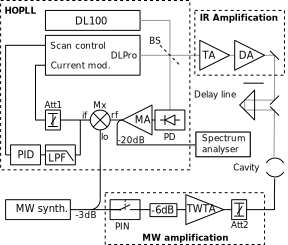
\includegraphics[width=\linewidth]{beatexp}

  \caption{Scheme of the experimental apparatus encompassing three different functions: Generating the amplitude modulated IR excitation laser, generating the microwave field with sufficient power, and phase-locking the envelope of the IR field on the microwave field as shown in Fig~\ref{fig:AMLaser}.
The AM IR laser is generated by the DL Pro and DL 100 lasers superimposed on the beamsplitter (BS), and then amplified by the IR amplification chain. The microwave is generated by a microwave synthesizer, formed into pulses by the PIN switch and amplified by the Traveling Wave Tube Amplifier (TWTA) before injection in the cavity.
 The locking of the IR field envelope with the microwave field is performed an Heterodyne Optical Phase Locked Loop denoted HOPLL on the figure.}
  \label{fig:exp_scheme}
\end{figure}


Fig.~\ref{fig:exp_scheme} shows the production of the amplitude modulated IR laser, the microwave, and the interplay between those two fields responsible for phase locking the envelope of the IR field with the microwave.


We are using two extended cavity diode lasers from Toptica, a DL 100 and a DL pro spaced in frequency by twice the microwave frequency. To create the beating the two lasers adjusted at the same power are superimposed on the BS 50:50 beamsplitter.

The first output seeds the IR amplification chain: About 15 mW is amplified to 800 mW by the TA tapered amplifier to seed the DA pulsed dye amplifier (LDS 819 in ethanol): Ultimately we obtain 20 ns long 6 $\mu$J pulses that are directed toward the microwave cavity after passing through an optical delay line. The pulse amplification degrades the linewidth of the IR lasers to about 100 MHz.

The second output of the BS beamsplitter is send to the PD fast photodiode (25 GHz bandwidth) which detects the 28 GHz beating note. In order to phase lock the laser beating note on the second harmonic of the microwave we are using a Heterodyne Optical Phase Locked Loop enclosed by the HOPLL rectangle in Fig.~\ref{fig:exp_scheme}.
 This beating signal is amplified by the MA low noise amplifier to be mixed on the Mx mixer with the second harmonic of the microwave synthesizer generated by the AD active frequency doubler. The intermediate frequency output (if) of the mixer is the error signal used in a dual loop correction scheme.


The shortest correction loop realizes a fast proportional correction, the error signal is directly sent to the current modulation input of the DL Pro, the Att1 attenuator adjusts the correction gain. The bandwidth of the correction is most likely limited by the current modulation characteristics of the diode. Using solely this loop, the system stays locked typically for dozens of seconds, which is too short for performing our measurements. The frequency correction allowed by current modulation is limited to a few megahertz to avoid mode hops, but our system is slowly drifting out of the correction frequency range causing unlocking. An important source of drifts is the master of the lock, the DL 100: it is free running and consequently drifts over a few megahertz on a minutes timescale, and proportional correction alone is known to lead to a non-null error. To extend the locking time we added a PID correction that handles low frequency deviations.

\begin{figure}[h]
  \centering
  \includegraphics[width=.6\linewidth]{stackSpec}
  \caption{Spectra of the laser beating note acquired by the spectrum analyzer shown in Fig.~\ref{fig:exp_scheme}. The frequency is offset by $2f_{mw}$.
Top: Laser beating signal locked at $2f_{mw}$ = 28 GHz (RBW: 1kHz, no averaging).
Bottom : Beating note spectra when the lasers are free running (RBW: 10 kHz, no averaging).}
  \label{fig:beat_spec}
\end{figure}
To realize the PID correction, the error signal is given to a Toptica PID110 PID trough the LPF 120 kHz low pass filter. This PID reinforces the correction at low frequency. Through the Toptica SC110 scan control, it acts on the diode current as well as the grating angle. This correction is slow but can follow DL 100 drifts of hundreds of megahertz without causing mode hops.
With those two loops working together we maintain continuous stable locks for several hours, greatly exceeding the 20 minutes needed to collect one data set.


Fig.~\ref{fig:beat_spec} shows spectra of the beating note before the mixer. On the bottom lies a spectrum acquired in the free-running case, on a second timescale it already shows a width of a few megahertz. Additionally the center of this spectra drifts by several megahertz in a 10 seconds timescale.
The top spectrum exhibits a strong and narrow peak at twice the microwave frequency ($2f_{mw}$) clearly showing that the system is locked. This central peak remains at the locking frequency as long as the system is locked. The two shoulders indicates a servo loop bandwidth about 1 MHz. The central peak is removed by 46 dB from the noise, and contains more than 99\% of the power. The -20 dB bandwidth of the central peak is below 2 kHz, this measurement being limited by the 1 kHz resolution bandwidth of our microwave spectrum analyzer. The overall performances of this system are sufficient for our use. Furthermore, the locking is routinely achieved in a couple of minutes and requires little maintenance.


\subsection{Microwave apparatus}
\label{sec:microwave-setup}
The microwave apparatus used is depicted on the bottom of Fig.~\ref{fig:exp_scheme}. The microwave source is a Hittite HMC T-2100 synthesizer tuned to the 14.007 GHz resonance of the cavity. Using a -3dB power spliter, half of its 11dBm cw output is used on the phase locked loop described above. The remainder is formed into 300 ns long pulses using the PIN PIN-diode switch and amplified by the TWTA Hughes 8020H04F traveling wave tube amplifier. Before the cavity the Att2 variable attenuator is used to adjust the microwave power injected in the cavity. The Fabry-Perot cavity is composed of two brass mirrors, each with 10 cm radius of curvature and 10.2 cm diameter, with a 7.85 cm on axis separation. Operated on TEM$_{007}$ mode, it has a quality Q of 3700, and we are able to determine the field in the cavity with an uncertainty of 15\%. A crucial aspect of the experiment is the reduction of stray electric fields, which ionize the high lying states we detect. To minimize stray fields, in addition to the plates above and below the cavity, we have installed metal plates on both sides as well. Bias voltages are applied to the plates and the cavity mirrors to reduce the stray fields to 1.5 mV/cm, estimated using the method described in \cite{Gurian_2010}.


%====================================================================================================
% \hrule
% In the experiment Li atoms in a beam pass through the antinode in the center of a 14 GHz Fabry-Perot cavity where they are optically excited by the route $2s\rightarrow 2p\rightarrow 3d\rightarrow nf,\epsilon f$. The first two transitions, at wavelengths 670 and 610 nm, are driven by pulsed dye laser beams which propagate along the axis of the microwave cavity. The third transition is driven by an amplitude modulated 819 nm pulsed laser beam which crosses the other two beams at a right angle at the central antinode of the microwave cavity, forming an excitation volume 1 mm on a side, much smaller than the microwave wavelength. The microwave field is turned off 10 ns after the last laser pulse, and after the laser and microwave pulses we field ionize bound atoms within 100 GHz of the limit by applying a negative voltage to a plate below the cavity. The freed electrons pass through a hole in a plate above the cavity en route to a dual microchannel plate detector. The signal from the microchannel plates is recorded by a gated integrator for later analysis. The laser pulses are 20 ns long, and the experiment is run at the 1 kHz repetition rate of the Nd:YLF pump laser.

% The essential idea of the recombination experiment is shown in Fig. \ref{fig:AMLaser}. The 819 nm laser beam is amplitude modulated synchronously with the microwave field in the cavity, as shown in Fig. 2. The laser field is given by :
% % \begin{equation}
% %   \label{eq:Eopt}
% %   E_{opt}(t)=E_o \sin \left( \omega_o t\right) \cos \left( \omega (t-t_0) \right)
% % \end{equation}


% By delaying the laser beam with an optical delay line we move the envelope of the laser field relative to the microwave field, altering the phase of the microwave field at which laser excitation occurs, as shown in Fig.~\ref{fig:AMLaser}. We record the field ionization signal from bound atoms as a function of the optical delay, or equivalently the phase of the microwave field at which excitation occurs.

% To produce the amplitude modulated beam described by  Eq.\eqref{eq:Eopt} and Fig.~\ref{fig:AMLaser} we combine the outputs of two continuous wave (cw) diode lasers operating at frequencies $\omega_o/2\pi\pm\omega/2\pi$. Phase locking of the envelope of the modulated laser beam to the microwave field is accomplished as follows. We detect the beat signal from the two lasers, at $2\omega/2\pi=28$ GHz, with a fast photodiode (25 GHz bandwidth). The beat signal is mixed with the second harmonic of the output of the microwave oscillator, producing an error signal which is applied to the tuning input of one of the diode lasers to complete the phase lock. With the two diode lasers adjusted to the same power, the resulting field envelope is as shown schematically in Fig.~\ref{fig:AMLaser}. The cw amplitude modulated beam is first amplified in a tapered amplifier and then in a pulsed dye amplifier, producing 20 ns long pulses.

% The microwave source is a Hittite HMC T-2100 synthesizer operating at 14.007 GHz. Approximately 5 mW of its cw output is frequency doubled and is used for phase locking the 819 nm lasers. The remainder, 5 mW, is formed into pulses 200 ns long using a PIN-diode switch and amplified by a Hughes 8020H04F traveling wave tube amplifier. The Fabry-Perot cavity is composed of two brass mirrors, each with 10 cm radius of curvature and 10.2 cm diameter, with a 7.85 cm on axis separation. Operated on TEM$_{007}$ mode, it has a Q of 3700, and we are able to determine the field in the cavity with an uncertainty of 15\%. A crucial aspect of the experiment is the reduction of stray electric fields, which ionize the high lying states we detect. To minimize them, in addition to the plates above and below the cavity  we have installed metal plates on both sides as well. Bias voltages are applied to the plates and the cavity mirrors to reduce the stray fields to 1.5 mV/cm.

\section{Results}
\label{sec:results}

\begin{figure}[h]
  \includegraphics[width=\linewidth]{phase_inversion}
  \caption{Rydberg state signal as a function of phase $\omega t_0$ between the microwave field and laser envelope for two different laser tunings: (a) $\omega_0/2\pi$ is 17 GHz below the ionization limit, (b) $\omega_0/2\pi$ is 25 GHz above the limit. In both cases the microwave field is $E_{mw}$ = 3 V/cm. The data (light gray) are fit to a sine function (black) to extract the peak-to-peak modulation. The total number of excited atoms  in $nf$ or $\epsilon f$ states is 1.00 on this scale. The phase origin for the horizontal scale is chosen to have the maximum energy transfer up and down at $\pi/6 $, in accordance with the results of our classical calculation.}
  \label{fig:e_signal}
\end{figure}
In Fig.~\ref{fig:e_signal} we show result of tuning the amplitude modulated 819 nm laser above and below the ionization limit. In both cases the Rydberg states are detected while scanning the optical delay as shown in Fig.~\ref{fig:AMLaser}. The vertical scale of the figure is relative to the total population promoted by the laser to $nf$ or $\epsilon f$ states.  In Fig.~\ref{fig:e_signal}b the center frequency $\omega_o/2\pi$ of the 819 nm laser is 25 GHz above the ionization limit, which is depressed by 7 GHz from its zero field value by the stray electric field. We see a large, 10 \% phase dependent modulation in the Rydberg state (recombination) signal. In Fig.~\ref{fig:e_signal}a $\omega_o/2\pi$ is tuned 17 GHz below the ionization limit, and the observed signal is inverted (shifted by $(0.26 \pm 0.1) \pi$) from that shown in Fig.~\ref{fig:e_signal}b. Since we are detecting Rydberg states, the inverted signal indicates that with the laser tuned below the limit ionization occurs at the same phase $\omega t_0$ as does recombination with the laser tuned above the limit, as expected from the classical model. Fig.~\ref{fig:e_signal} shows two important features. First, we observe both energy transfer to the electron, as in the He experiments, and from the electron, as in the ps-microwave experiment. Second, the magnitude of the phase modulation, $\simeq 10\%$,  is far greater than that observed with single ps laser pulse excitation.

In Fig.~\ref{fig:e_modulation} we plot the observed modulation amplitudes for the tunings of Fig.~\ref{fig:e_modulation} vs the microwave field as well as those calculated using a classical  model. The modulation in Fig.~\ref{fig:e_modulation}a is plotted as negative to indicate the phase reversal shown in Fig.~\ref{fig:e_signal}. In Fig.~\ref{fig:e_modulation}b, with the laser tuned above the limit, the experimental modulation signal increases to a maximum at $E_{mw}=2.5$ V/cm and decreases to zero at 5 V/cm. In Fig.~\ref{fig:e_modulation}a the signal again increases to a maximum at 3 V/cm, but, unlike Fig.~\ref{fig:e_modulation}b, slowly decreases as the field is raised, never reaching zero.

It is instructive to compare the observed dependence of the modulation on the microwave field to the results of a one dimensional classical model. In the model an electron near the ionization limit is launched from the center of a soft core coulomb potential at the phase $\omega t_0$ of the microwave field\cite{Eberly_1992}. We calculate numerically the classical motion of the electron to find the phase dependent probability of its returning to the ionic core on its first orbit, ignoring later orbits. Since the coulomb potential, not the microwave field, reflects the electron, it returns to the core with a negative total energy. It worth noting that we calculate the motion of an electron within only one orbit, but, as illustrated in Fig.~\ref{fig:Wexchange}, this orbit occurs over multiple microwave cycles. To avoid confusion, in the following 'orbit' refers to the electronic motion whereas 'cycle' refers to the microwave field. In Fig.~\ref{fig:e_modulation}b the laser tuning in the model is 25 GHz above the limit. There is no recombination until its onset at $E_{mw}$=2.5 V/cm, when the maximum energy transfer of Eq.~\eqref{eq:magW} equals the laser tuning above the limit. At this field recombination occurs only at the phases $\omega t_0 \simeq \pi/6$ and $7\pi/6$. As the field is raised recombination occurs over a widening phase interval, and the maximum modulation occurs when recombination occurs over the phase intervals $\pi/6-\pi/4\lesssim \omega t_0\lesssim \pi/6+\pi/4$ and $7\pi/6-\pi/4\lesssim \omega t_0\lesssim 7\pi/6+\pi/4$, which is, not surprisingly, when recombination occurs half the time. In Fig.~\ref{fig:e_modulation}b this occurs at $E_{mw}$=3 V/cm. As $E_{mw}$ is further increased the fraction of time during which recombination occurs increases, and the modulation slowly decreases. The calculated modulation shown in Fig.~\ref{fig:e_modulation}a is essentially the same.


\begin{figure}[h]
  \includegraphics[width=.9\linewidth]{modulation}
  \caption{Peak-to-Peak modulation of the Rydberg states signal as a function of microwave field $E_{mw}$ when the laser is tuned (a) 17 GHz below and (b) 25 GHz above the ionization limit. The experimental data points have error bars and the results of a classical calculation are shown as broken lines. The negative modulation in (a) reflects the phase inversion between Fig.~\ref{fig:e_signal}(a) and Fig.~\ref{fig:e_signal}(b). Note the factor of three difference in the two vertical scales.}
  \label{fig:e_modulation}
\end{figure}

\section{Discussion}
\label{sec:discussion}
The classical model provides useful insights into the experimental data. First, we note that at fields above 3 V/cm the model predicts a slow decrease in the modulation, which is observed in Fig. 6a, but not in Fig. 6b. It is not observed in Fig. 6b because an electron which has been recombined on the first orbit, the only orbit considered in the model, can be ionized on a subsequent orbit, obliterating the modulation. In contrast, in Fig. 4a an electron ionized on the first orbit remains ionized; there are never any subsequent orbits. Thus Fig. 6a can be expected to match reasonably well a single orbit model, and, aside from the overall scale factor, it does. The discrepancy between the model and the experimental results in Fig. 6b at fields above 3 V/cm is evidently due to ignoring later orbits, when ionization can reduce the number of Rydberg states remaining to be detected.

There are two differences between the model and the experiment at low microwave fields. First, in both Figs. \ref{fig:e_modulation}a and \ref{fig:e_modulation}b the experimentally observed modulation rises more slowly than does the calculated modulation. Second, in Fig.~\ref{fig:e_modulation}b the onset of the modulation occurs before it is classically allowed one of the hallmarks of a quantum mechanical process. While tunneling is the most familiar of such processes, a resonant transition driven by multiple field cycles is another\cite{Stoneman_1988}.

The notion that multiple field cycles are important is the motivation for Floquet approaches to this and similar problems\cite{Tong_2010,Murakami_2013,Chu_1977,Giutsi_1987}. Further support for a Floquet approach comes from frequency domain experiments, in which series of peaks above the limit, separated by the microwave frequency, were observed\cite{Shuman_2008,Gurian_2010,Arakelyan_2014}, as well as from the phase dependence reported here. Since the amplitude modulated laser field has only two optical frequency components, the relation between the relative phases of the two optical components at $\omega_0 \pm \omega$ and the phase of the envelope is particularly  simple. A phase shift of $\omega t_0$ in one of the components shifts the envelope by $\omega t_0/2$. Delaying the envelope is equivalent to shifting the phase of one of the two components. The observed phase dependence in Fig.~\ref{fig:e_signal} and Fig.~\ref{fig:e_modulation} is thus indicative of coherent excitation of Floquet sidebands at $\omega_o\pm\omega$, as suggested previously\cite{Tong_2010}.

While the classical one orbit model is intuitively appealing, it overstimates the amplitude of the modulation by at least a factor of three, as shown by Fig. 4. We attribute this discrepancy to two factors. First, small, 1.5 mV/cm, stray fields field ionize the high lying states, reducing the size of all signals. 
Second, the model ignores the effect of later microwave cycles, which lead to more ionization, reducing the total detected signal, and the modulation as well.

\section{Conclusion}
\label{sec:conclusion}
In conclusion, the enormous increase in the phase dependent modulation signal when the laser excitation occurs over multiple microwave cycles, as opposed to during a single cycle~\cite{Overstreet_2011}, demonstrates experimentally the importance of coherence in the excitation, as predicted in He APT-IR laser calculations~\cite{Johnsson_2005}. Furthermore, the energy transfer is much larger than expected on the basis of the microwave field alone, due to the presence of the coulomb potential. For the same reason, in APT-IR experiments analogous energy transfer effects will be important even in relatively weak IR fields.

\begin{acknowledgments}
It is a pleasure to acknowledge useful discussions with R. R. Jones. This work has been supported by the U. S. Department of Energy, Chemical Sciences Division.  
\end{acknowledgments}


\bibliography{biblio}
%\bibliographystyle{natbib}


\end{document}
%%% Local Variables:
%%% mode: latex
%%% TeX-master:
%%% End:
